\chapter{Software}

\section{Overview}
\label{sec:software-overview}
The software component of the amplifier system will be running on top of an embedded real-time operating system (such as FreeRTOS). This operating system will provide the task management and scheduling required by the rest of the application. The main software components are shown in \autoref{fig:diagram}; a description of each can be found in the following sections. Along with each component, a list of publicly-available functions for that component is listed. This helps better define the software interface requirements that will be used by the other modules in the system.

\begin{figure}[H]
	\centering
	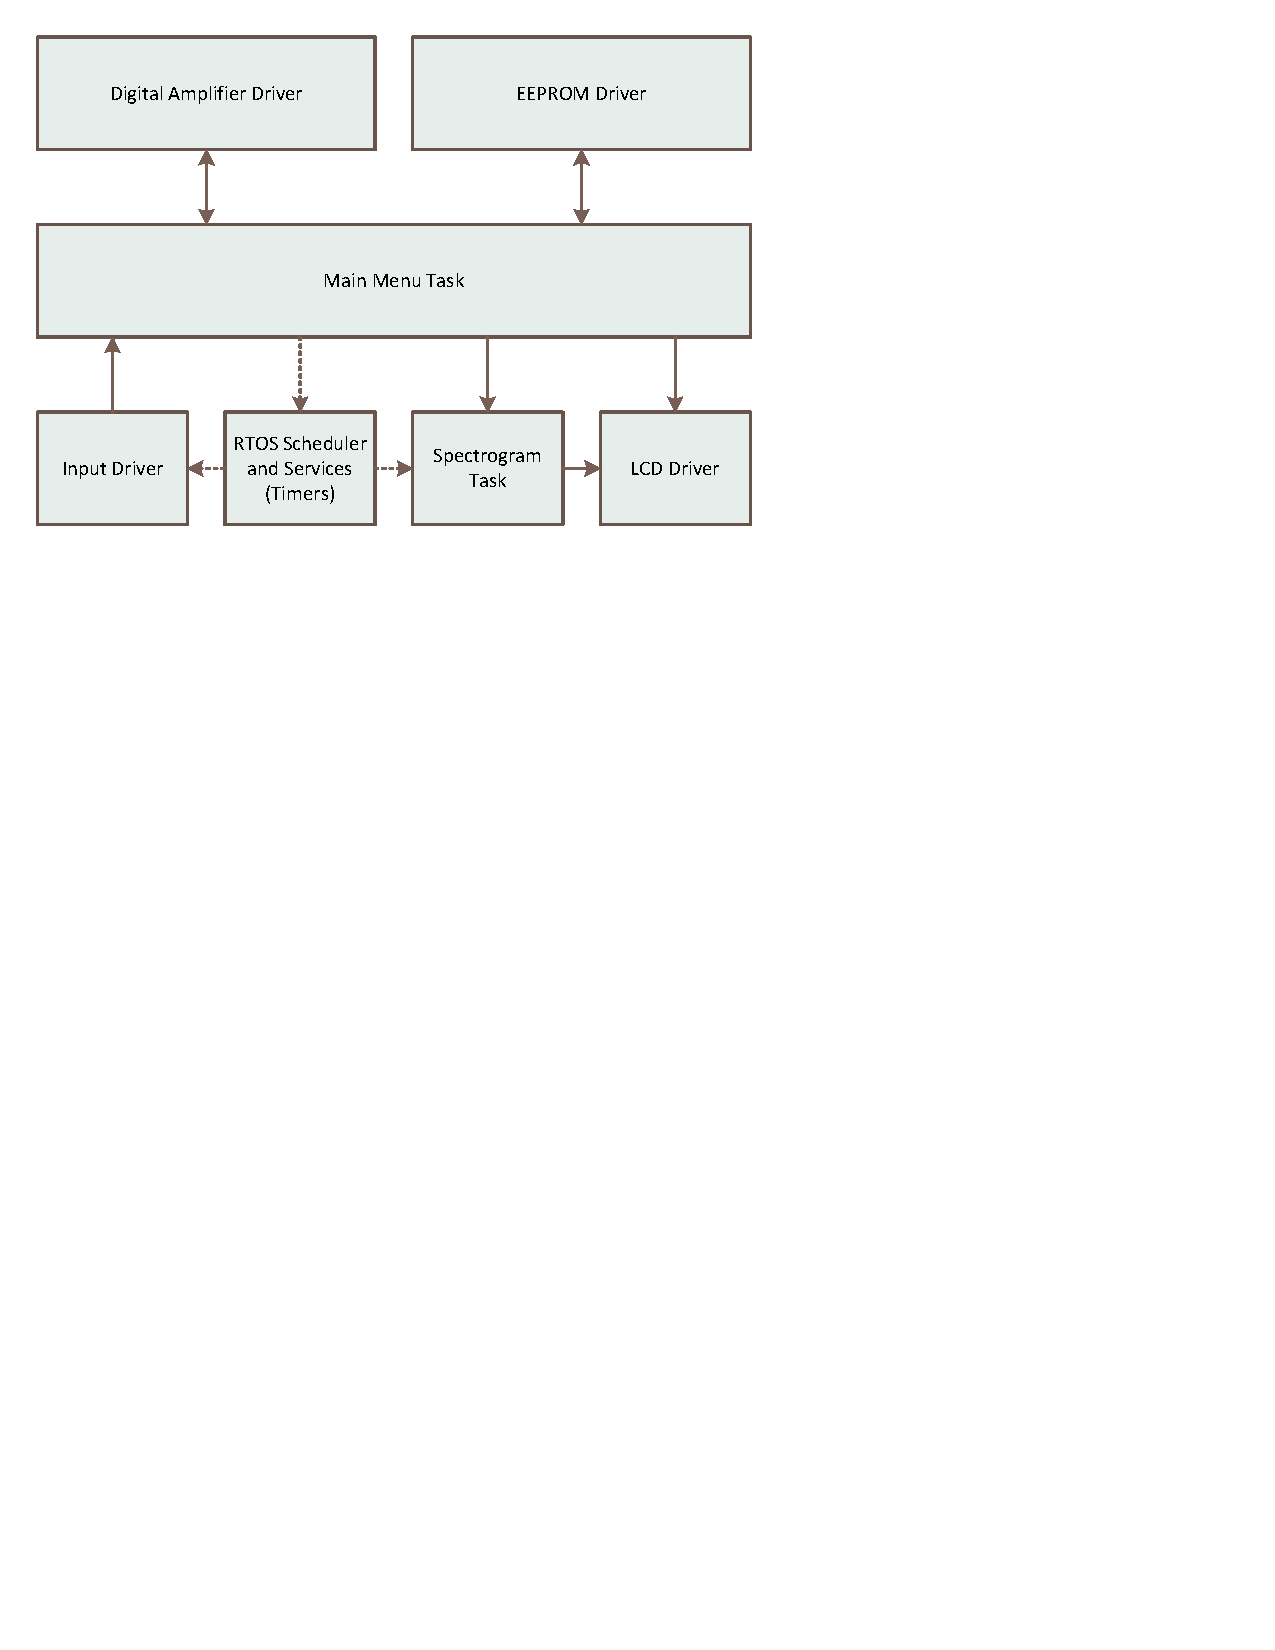
\includegraphics{diagram}
	\caption[Software Componenent Overview]%
	{Overview of the software components of the Digital Amplifier system.}
	\label{fig:diagram}
\end{figure}

\section{Input Drivers (Buttons and Scroll Wheel)}
\label{sec:io-driver}
The functionality of the wheel and buttons are described in \autoref{sec:rotary} and \autoref{sec:buttons}. The high-level button and scroll wheel functions will be actuated through RTOS events which will allow the functions to be reassigned based on the state of the interface. There will be one function assigned for each of the buttons as well as one for each the \emph{Up} and \emph{Down} motions of the scroll wheel.

\section{Digital Amplifier Driver}
\label{sec:amp-driver}
The CS4525 uses I\superscript{2}C and a series of single-byte configuration registers for all of its communications. The \emph{Reset} line is used to control power to the amplifier and is only used in initialization and in the case of error conditions. The core functions of this driver therefore are only those for single-byte reads and writes, as well as interrupt handling. Ur

\subsection*{Functions}
\begin{itemize}
\item \verb|void amp_init(void)|

Initializes I\superscript{2}C channel 1 and loads default values.

\item \verb|void amp_write_byte(char addr, char value)|

Sets a byte in the amplifier registers.

\item \verb|char amp_read_byte(char addr)|

Reads a byte in the amplifier registers.
\end{itemize}

\section{EEPROM Driver}
\label{sec:eeprom-driver}
The EEPROM is very simple in function, using a buffer to allow writing of up to 128 bytes at a time. The microprocessor communicates with the EEPROM using an I\superscript{2}C interface. This functionality is further described in \autoref{sec:eeprom}

\subsection*{Functions}
\begin{itemize}
\item \verb|void e2p_init(void)|

Initializes I\superscript{2}C channel 2.

\item \verb|void e2p_write_byte(char addr, char value)|

Writes a single byte to the EEPROM.

\item \verb|char e2p_read_byte(char addr)|

Reads a single byte from the EEPROM.

\item \verb|char e2p_write(char addr, char len, char* buf)|

Writes an arbitrary amount of data to the EEPROM and returns the count.

\item \verb|char e2p_read(char addr, char len, char* buf)|

Reads an arbitrary amount of data from the EEPROM and returns the count.
\end{itemize}

\section{LCD Driver}
\label{sec:lcd-driver}
The LCD driver is controlled using a list of functions that write to the LCD board in different ways. There is a function that writes a new line, a function that writes to a specified column and row, there is a function that writes a single character, a function that can write a single byte, and a function that can clear the screen so that more data can be written to it. The purpose of having all of these different ways to manipulate the LCD screen is two-fold. One, the various functions for writing to the LCD allowed for greater control over the way the user interface is designed. The functionality provided by the LCD interface allows us to implement features like writing non-ASCII characters to the screen (necessary to provide the ability to show a visualization when no music is playing). Second, we can use many of these functions during testing to ensure that the LCD board, and the modules connected to it functioned properly. Additionally the brightness and contrast can be controlled by using a PWM signal. There are additional software functions for controlling these variables by generating different pulse widths for each of these variables based on settings defined through the menu system. These functions together provide a driver interface for the rest of the software to use.

Timing is an issue when writing to LCD; to avoid complexity, we have chosen to make these functions block and use timed poll loops instead of deferring execution to the scheduler. This could later be transparently changed if performance is an issue.

\subsection*{Functions}
\begin{itemize}
\item \verb|void lcd_init(void)|

Initializes communication with the LCD device.

\item \verb|void lcd_clear(void)|

Clears the LCD display.

\item \verb|void lcd_print(uchar line, uchar col, const char *fmt, ...)|

Writes the specified format string to the appropriate position on the LCD.
\end{itemize}

\section{User Interface}
\label{sec:ui}

One of the more important software design issues that we needed to consider was the user interface (UI). When designing any system that is user-controlled, it is crucial to design a UI that is both simple and effective. We have chosen to make the interface based on a state machine implemented in an event-driven manner, similar to many real-time systems. The structure of this state machine is described in more detail below.

Initially, the system is in the \emph{Main} state. In this state, a user can control the volume using the knob, and the LCD will display the volume level. This display times out after 10 seconds.

As described in \autoref{sec:buttons}, the system also has four available buttons. In any state, the bottom button (the home button) will cause the system to return to the \emph{Main} state. This provides the user with a quick way to exit any menu. The top left button (the mute button) will also work in every state, and will cause the system to either mute or unmute the audio output. The top middle button (the menu/select button) will cause a state-dependent transition corresponding to ``selecting'' a menu option or entering the main menu. The last button (the back button) will take the user to the previous menu. There will be an inactivity timeout (which can be chosen by the user, but defaulted at 30 seconds) after which the system will go back to the \emph{Main} state.

The menu structure corresponds directly to the states in the state machine. These are shown in their logical structure below.

\begin{itemize}

\item \textbf{(M)} Sound
\begin{itemize}
	\item \textbf{(C)} Freq1 (Bass)
	\item \textbf{(C)} Freq2
	\item \textbf{(C)} Freq3 (Mid)
	\item \textbf{(C)} Freq4
	\item \textbf{(C)} Freq5 (Treble)
	\item \textbf{(B)} Enable/Disable Adaptive Loudness Compensation
\end{itemize}

\item \textbf{(M)} System
\begin{itemize}
	\item \textbf{(B)} Enable/Disable Spectrum Analyzer
	\item \textbf{(C)} Screen Contrast
	\item \textbf{(C)} Screen Brightness
\end{itemize}

\item \textbf{(M)} Presets
\begin{itemize}
	\item \textbf{(M)} Load Preset
	\begin{itemize}
		\item \textbf{(A)} Preset 1
		\item \textbf{(A)} Preset 2
		\item \textbf{(A)} Preset 3
	\end{itemize}

	\item \textbf{(M)} Save Preset
	\begin{itemize}
		\item \textbf{(A)} Preset 1
		\item \textbf{(A)} Preset 2
		\item \textbf{(A)} Preset 3
	\end{itemize}
\end{itemize}

\end{itemize}

In this menu description, \textbf{(M)} corresponds to a menu or submenu. When the system is in one of these states, the scroll wheel allows the user to select an appropriate item in the menu, and the menu button activates the selected item. The back button navigates up to the parent state in the tree. \textbf{(B)} corresponds to a boolean option; when activated by pressing the menu button, the option is either enabled or disabled, and the system remains in the same state. \textbf{(C)} represents a continuous parameter; when activated, this displays a value and a graphical indicator of the present value on the LCD. From this state, scrolling the wheel changes the parameter value, and pressing either of the back or menu buttons causes the system to return to the previous state. \textbf{(A)} is an action; when selected, the system performs the appropriate action and returns to the \emph{Main} state.

\section{Spectrogram}
\label{sec:spectrogram}
While the system is idle, a spectrogram will be played on the screen, displaying frequency-domain power spectrum of the output signal. This uses the logic-level PWM output from the amplifier for a single channel as its input source. As this feature is a novelty and the LCD refresh rate is rather low, the computation of this spectrum only needs to occur about 10 times per second and only when on the main screen. The spectrogram uses data sampled using the \emph{Input Capture} module on the controller, capturing a low-resolution signal at approximately 300kHz. At this rate, 256 samples will be used for each spectrum, with each of the 16 spectrogram bins being summed over 8 DFT bins. The system will use the Goertzel DFT algorithm, which allows the assignment of arbitrary bin values so that the frequency spectrum can be shown on a logarithmic scale.  

\subsection*{Functions}
\begin{itemize}
\item \verb|void spectrogram(void)|

Runs the spectrogram task.
\end{itemize}

\section{Main Task}

The main task will be the initial one started by the real-time operating system, in charge of handling communication between the individual subsystems as well as displaying the menu.

When entering the \emph{Main} (initial) state, the menu task will (depending on the user's configuration settings) launch the spectrogram task (\autoref{sec:spectrogram}) and display additional status information on the LCD. Here it will wait for a button to be pressed or (if muted) a timeout to occur. Inside the menus it will wait for either a timeout (to return to the \emph{Main} state) or a button press (and perform the appropriate action as described in \autoref{sec:ui}).

\subsection*{Functions}
\begin{itemize}
\item \verb|void main(void)|

Initializes the entire system and then runs the menu task.

\item \verb|void menu(void)|

Runs the state machine for the user interface described in \autoref{sec:ui} as a task.
\end{itemize}
